\let\negmedspace\undefined
\let\negthickspace\undefined
\documentclass[journal]{IEEEtran}
\usepackage[a5paper, margin=10mm, onecolumn]{geometry}
%\usepackage{lmodern} % Ensure lmodern is loaded for pdflatex
\usepackage{tfrupee} % Include tfrupee package

\setlength{\headheight}{1cm} % Set the height of the header box
\setlength{\headsep}{0mm}     % Set the distance between the header box and the top of the text

\usepackage{gvv-book}
\usepackage{gvv}
\usepackage{cite}
\usepackage{amsmath,amssymb,amsfonts,amsthm}
\usepackage{algorithmic}
\usepackage{graphicx}
\usepackage{textcomp}
\usepackage{xcolor}
\usepackage{txfonts}
\usepackage{listings}
\usepackage{enumitem}
\usepackage{mathtools}
\usepackage{gensymb}
\usepackage{comment}
\usepackage[breaklinks=true]{hyperref}
\usepackage{tkz-euclide} 
\usepackage{listings}
% \usepackage{gvv}                                        
\def\inputGnumericTable{}                                 
\usepackage[latin1]{inputenc}                                
\usepackage{color}                                            
\usepackage{array}                                            
\usepackage{longtable}                                       
\usepackage{calc}                                             
\usepackage{multirow} 
\usepackage{hhline}                                           
\usepackage{ifthen}                                           
\usepackage{lscape}
\usepackage{circuitikz}
\tikzstyle{block} = [rectangle, draw, fill=blue!20, 
    text width=4em, text centered, rounded corners, minimum height=3em]
\tikzstyle{sum} = [draw, fill=blue!10, circle, minimum size=1cm, node distance=1.5cm]
\tikzstyle{input} = [coordinate]
\tikzstyle{output} = [coordinate]

\begin{document}
\bibliographystyle{IEEEtran}
\vspace{3cm}

\title{MatGeo Assignment 6.4.7}
\author{AI25BTECH11007}
 \maketitle
% \newpage
% \bigskip
{\let\newpage\relax\maketitle}

\renewcommand{\thefigure}{\theenumi}
\renewcommand{\thetable}{\theenumi}
\setlength{\intextsep}{10pt} % Space between text and floats


\numberwithin{equation}{enumi}
\numberwithin{figure}{enumi}
\renewcommand{\thetable}{\theenumi}
\noindent
\textbf{Question :}\\
Two motorcycles A and B are running at a speed more than the allowed speed on
the road represented by the following lines:
\[
\mathbf{r} = \lambda(\mathbf{i} + 2\mathbf{j} - \mathbf{k}), \qquad
\mathbf{r} = (3\mathbf{i} + 3\mathbf{j}) + \mu(2\mathbf{i} + \mathbf{j} + \mathbf{k}).
\]

Based on the following information, answer the questions:

\begin{enumerate}
    \item Find the shortest distance between the given lines.
    \item Find a point at which the motorcycles may collide.
\end{enumerate}

\noindent\\
\textbf{Solution :}
Let $\vec{x}_1$ and $\vec{x}_2$ be the points on the given lines respectively.
\[
\vec{x}_1 = \lambda\myvec{1\\2\\-1}, \qquad 
\vec{x}_2 = \myvec{3\\3\\0} + \mu\myvec{2\\1\\1}
\]

\noindent\\
\textbf{(a) Shortest distance:}\\
Let $\vec{A} = \myvec{0\\0\\0}$ and $\vec{B} = \myvec{3\\3\\0}$

Let
\[
\vec{M} = \myvec{1 & 2 \\ 2 & 1 \\ -1 & 1}
\]

\begin{equation}
    (\vec{M} \, \, \vec{B}-\vec{A}) = \myvec{1 & 2 & 3 \\ 2 & 1 & 3 \\ -1 & 1 & 0}
\end{equation}

Row Transformation-1: $R_2 \rightarrow R_2 - 2R_1$
\begin{equation}
\myvec{1 & 2 & 3 \\ 0 & -3 & -3 \\ -1 & 1 & 0}
\end{equation}

Row Transformation-2: $R_3 \rightarrow R_3 + R_1$
\begin{equation}
\myvec{1 & 2 & 3 \\ 0 & -3 & -3 \\ 0 & 3 & 3}
\end{equation}

Row Transformation-3: $R_3 \rightarrow R_3 + R_2$
\begin{equation}
\myvec{1 & 2 & 3 \\ 0 & -3 & -3 \\ 0 & 0 & 0}
\end{equation}

Therefore, \(\operatorname{rank}=2 < 3 \Rightarrow\) The Lines intersect (not skew).

\begin{align}
    \boxed{\text{The Shortest Distance between the given Lines = } 0 \text{ units}}
\end{align}

\textbf{(b) Intersection Point:} 

At intersection, the points on the lines are equal:
\[
\vec{x}_1 = \vec{x}_2 \quad \Longrightarrow \quad
\lambda\myvec{1\\2\\-1} = \myvec{3\\3\\0} + \mu\myvec{2\\1\\1}
\]

Equating components gives a system of equations:
\[
\begin{cases}
\lambda - 2 \mu = 3 \\[1mm]
2 \lambda - \mu = 3 \\[1mm]
- \lambda - \mu = 0
\end{cases}
\]

Write in augmented matrix form:
\[
\left[\begin{array}{rr|r}
1 & -2 & 3 \\[1mm]
2 & -1 & 3 \\[1mm]
-1 & -1 & 0
\end{array}\right]
\]

Row Reduction-1 : $R_2 \rightarrow R_2 - 2 R_1$
\[
\left[\begin{array}{rr|r}
1 & -2 & 3 \\[1mm]
0 & 3 & -3 \\[1mm]
-1 & -1 & 0
\end{array}\right]
\]

Row Reduction-2 : $R_3 \rightarrow R_3 + R_1$
\[
\left[\begin{array}{rr|r}
1 & -2 & 3 \\[1mm]
0 & 3 & -3 \\[1mm]
0 & -3 & 3
\end{array}\right]
\]

Row Reduction-3 : $R_3 \rightarrow R_3 + R_2$
\[
\left[\begin{array}{rr|r}
1 & -2 & 3 \\[1mm]
0 & 3 & -3 \\[1mm]
0 & 0 & 0
\end{array}\right]
\]

From $R_2$: $3 \mu = -3 \implies \mu = -1$ \\
From $R_1$: $\lambda - 2(-1) = 3 \implies \lambda + 2 = 3 \implies \lambda = 1$

\[
\therefore \lambda = 1, \quad \mu = -1
\]

Intersection point:
\[
\vec{r} = \lambda \myvec{1\\2\\-1} = \myvec{1\\2\\-1}
\]

\[
\vec{r} = \myvec{3\\3\\0} + \mu \myvec{2\\1\\1} = \myvec{1\\2\\-1}
\]

\[
\boxed{\text{Intersection Point = } (1,\,2,\,-1)}
\]

\begin{figure}[H]
    \centering
    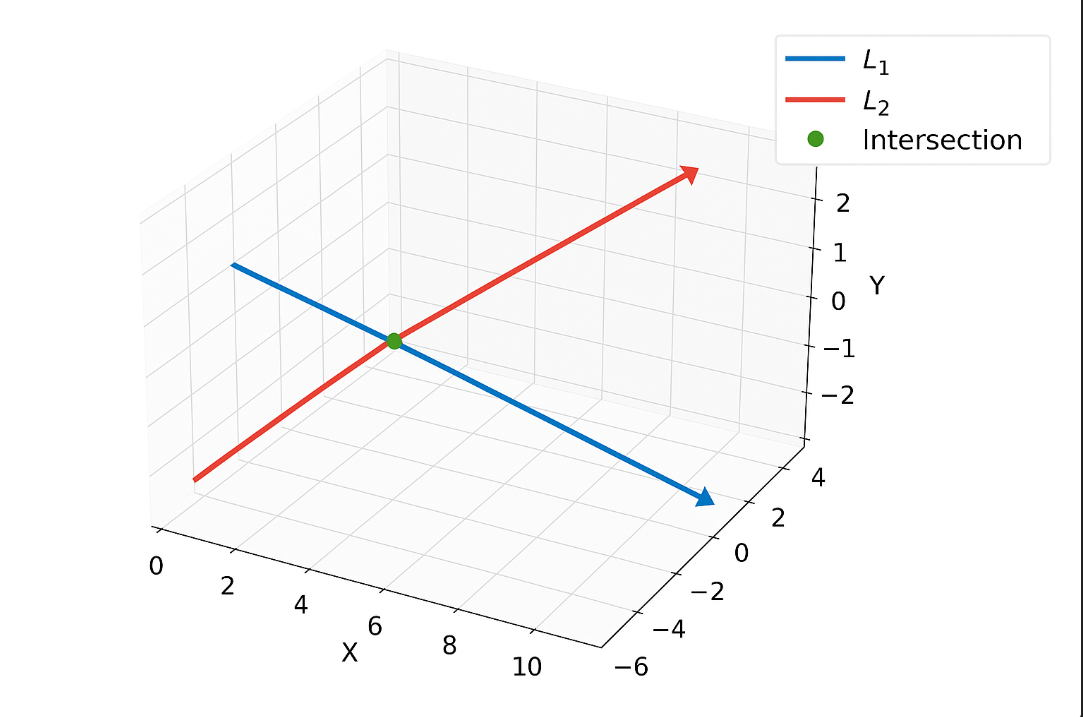
\includegraphics[width=0.75\linewidth]{figs/image.png}
    \caption{Image}
    \label{fig:placeholder}
\end{figure}


\end{document}
